\chapter{Preliminaries}\label{chapter:background}
This chapter introduces \acrlong{abe} and the relevant mathematical background for implementing it.


\begin{figure} \centering
    \begin{subfigure}{.8\textwidth}
        \begin{tikzpicture}
            \draw[->] (0, 0) node [anchor=east] {m} -- ++(1, 0) node (encrypt) [anchor=west, draw] {Encrypt};
            \path (encrypt.north) -- +(0, 0.3) pic [anchor=west, scale=0.1, red, fill=red] {key};
            \draw[->] (encrypt.east) -- ++(2, 0) node [anchor=south] {c} -- ++(2,0) node (decrypt) [anchor=west, draw] {Decrypt};
            \path (decrypt.north) -- +(0, 0.3) pic [anchor=west, scale=0.1, red, fill=red] {key};
            \draw[->] (decrypt.east) -- ++(1,0) node [anchor=west] {m};
        \end{tikzpicture}
        \caption{Symmetric Encryption: The same key is used for encryption and decryption. This key needs to be kept secret.} \label{fig:keys-symmetric}
    \end{subfigure}
    \\
    \vspace{0.5cm}
    \begin{subfigure}{.8\textwidth}
        \begin{tikzpicture}
            \draw[->] (0, 0) node [anchor=east] {m} -- ++(1, 0) node (encrypt) [anchor=west, draw] {Encrypt};
            \path (encrypt.north) -- +(0, 0.3) pic [anchor=west, scale=0.1, olive, fill=olive] {key};
            \draw[->] (encrypt.east) -- ++(2, 0) node [anchor=south] {c} -- ++(2,0) node (decrypt) [anchor=west, draw] {Decrypt};
            \path (decrypt.north) -- +(0, 0.3) pic [anchor=west, scale=0.1, red, fill=red] {key};
            \draw[->] (decrypt.east) -- ++(1,0) node [anchor=west] {m};
        \end{tikzpicture}
        \caption{Asymmetric Encryption: Different keys for encryption and decryption. Decryption succeeds if and only if the decryption key is exactly the counterpart to the encryption key. Only the decryption key needs to be kept secret.} \label{fig:keys-asymmetric}
    \end{subfigure}
    \\ 
    \vspace{0.5cm}
    \begin{subfigure}{.8\textwidth}
        \begin{tikzpicture}[sibling distance=4mm, level distance=3mm]
            \draw[->] (0, 0) node [anchor=east] {m} -- ++(1, 0) node (encrypt) [anchor=west, draw] {Encrypt};
            
            \scoped{
                \tikzstyle{every node}=[fill, circle, draw, inner sep=0.5mm];
                \tikzstyle{level 2}=[sibling distance=1.5mm];
                \fill[red] (decrypt.north) -- ++(0, 0.7) node [anchor=south] {} child {node {} child {node {}} child {node {}} child {node {}}} child { node {} child {node {}}};
            };
            \draw[->] (encrypt.east) -- ++(2, 0) node [anchor=south] {c} -- ++(2,0) node (decrypt) [anchor=west, draw] {Decrypt};
            \path (encrypt.north) -- +(0, 0.3) node [olive] {$\{A, B, C\}$};
            \draw[->] (decrypt.east) -- ++(1,0) node [anchor=west] {m};
        \end{tikzpicture}
        \caption{\glslink{gls-kp-abe}{Key-Policy Attribute-Based Encryption}: Attributes for encryption, access structure for decryption. Decryption succeeds if and only if the attributes of the ciphertext satisfy the policy embedded in the key.} \label{fig:keys-abe}
    \end{subfigure}
    \\ 
    \vspace{0.5cm}
    \begin{subfigure}{.8\textwidth}
        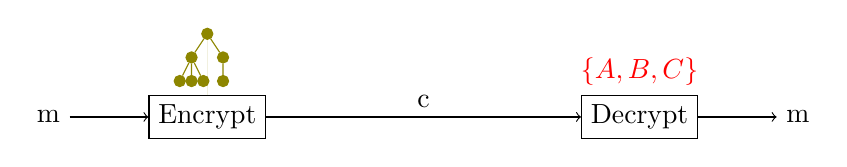
\begin{tikzpicture}[sibling distance=4mm, level distance=3mm]
            \draw[->] (0, 0) node [anchor=east] {m} -- ++(1, 0) node (encrypt) [anchor=west, draw] {Encrypt};
            
            \scoped{
                \tikzstyle{every node}=[fill, circle, draw, inner sep=0.5mm];
                \tikzstyle{level 2}=[sibling distance=1.5mm];
                \fill[olive] (encrypt.north) -- ++(0, 0.7) node [anchor=south] {} child {node {} child {node {}} child {node {}} child {node {}}} child { node {} child {node {}}};
            };
            \draw[->] (encrypt.east) -- ++(2, 0) node [anchor=south] {c} -- ++(2,0) node (decrypt) [anchor=west, draw] {Decrypt};
            \path (decrypt.north) -- +(0, 0.3) node [red] {$\{A, B, C\}$};
            \draw[->] (decrypt.east) -- ++(1,0) node [anchor=west] {m};
        \end{tikzpicture}
        \caption{\glslink{gls-cp-abe}{Ciphertext-Policy Attribute-Based Encryption}: \Gls{access-policy} for encryption, attributes for decryption. Decryption succeeds if and only if the attributes of the key match the policy embedded in the ciphertext.} \label{fig:keys-abe}
    \end{subfigure}
    \caption[Keys in different classes of encryption schemes]{Keys used for encryption and decryption in different classes of encryption schemes. Red information has to be kept secret, green information may be made publicly available. For the differences between the two types of \acrshort{abe}, see section~\ref{sec:cp-vs-kp}.}
    \label{fig:key-use}
\end{figure}

\section{Confidentiality with Classic Symmetric and Asymmetric Cryptography}
Today's conventional cryptography knows two main classes of encryption schemes: \glslink{privkes}{symmetric} and \glslink{pkes}{asymmetric encryption}. See Figure~\ref{fig:key-use} for an illustration of the differences.

Consider $n$ participants wanting to communicate securely (i.e. no user can read encrypted messages between two other users).
Using a \gls{privkes}, each participant would need to agree on a unique key with every other participant, resulting in a total number of $\frac{n(n-1)}{2}$ keys.
The users would need to exchange these keys secretly, e.g. by meeting in person.
Using an \gls{pkes} removes the need for secret key exchange because the encryption keys can be published.
It also reduces the total number of keys to only $n$, because each participant could obtain every other participant's public key and use it to send them encrypted messages.

Another problem remains, however: Encrypting a single message to several recipients requires encrypting it with everyone's public key separately.
For a large number of recipients, this is inefficient:
To encrypt a message for all students of a certain university, we would need to obtain each student's public key and encrypt the message with each key separately.

Even worse, what if we want to encrypt data for any student of said university, even if they \emph{haven't joined the university yet}?
In this case, our only option using classic cryptography would be to have some trusted instance keep a plaintext copy and re-encrypt the data for any new student when they join the university.
Attribute-Based encryption solves this problem.

\section{Attribute-Based Encryption}\label{sec:background-abe}
\acrfull{abe} uses a combination of attributes to define a \emph{group} of private keys that should be able to read encrypted data, instead of encrypting it for one specific private key only (as in \glspl{pkes}).
In Figure~\ref{fig:key-use}, this is represented by a tree.

The combination of attributes may be as restrictive or permissive as needed.
It is possible to create ciphertexts that can be read by almost all members of an \acrshort{abes}, and ciphertexts that can be read by nobody except a few selected participants.

Figure~\ref{fig:abe-system} shows how the participants interact in a small \acrshort{abe} system.
Details are explained in the following sections.

\subsection{Attributes and the Key Generation Center}\label{sec:kgc}

\begin{figure}
    \centering
    \begin{subfigure}[t]{0.45\textwidth}
        \centering
        \begin{tikzpicture}[actor/.style={draw, minimum width=1.5cm}]
            \node[actor] (a) at (-1,0) {Alice};
            \node[actor] (b) at (1,0) {Bob};
            \node[actor] (kgc) at (0,1.5) {KGC};
        
            \node[above, align=center] at (kgc.north) {$\{PK, MK\}:=\text{Setup}()$};

            \node[below, align=center] at (a.south) {$\{m, \omega\}$\\};
            \node[below, align=center] at (b.south) {$\{\}$};

            % \draw[->] (a) edge node[left] {\{$S_A$\}} (kgc);
            % \draw[->] (b) edge node [right] {\{$S_B$\}} (kgc);
            % \draw[->] (a) edge pic [left=0.5cm, scale=0.05] {key} node [left=.5cm] {k} (kgc);
            \draw[->] (b) edge pic [right=0.5cm, scale=0.5, blue] {tree} node [right=.75cm, blue] {$S_B$} (kgc);
            % TODO fix arrows
            \draw[->] (a) edge pic [left=0.5cm, scale=0.5, olive] {tree} node [left=.75cm, olive] {$S_A$} (kgc);
            % \draw[->] (b) edge node [right] {\{$S_B$\}} (kgc);

        \end{tikzpicture}
        \caption{Setup phase I: Generation of Parameters}
    \end{subfigure}
    ~
    \begin{subfigure}[t]{0.45\textwidth}
        \centering
        \begin{tikzpicture}[actor/.style={draw, minimum width=1.5cm}]
            \node[actor] (a) at (-1,0) {Alice};
            \node[actor] (b) at (1,0) {Bob};
            \node[actor] (kgc) at (0,1.5) {KGC};

            \node[above, align=center] at (kgc.north) {$\{PK, MK\}$\\$\textcolor{olive}{k_A} := \text{KeyGen}(MK, \textcolor{olive}{S_A})$\\$\textcolor{blue}{k_B} := \text{KeyGen}(MK, \textcolor{blue}{S_B})$};

            \node[below, align=center] at (a.south) {{\{$PK$, $\textcolor{olive}{k_A}$\}}\\$\{m, \omega\}$};
            \node[below, align=center] at (b.south) {\{$PK$, $\textcolor{blue}{k_B}$\}};

            \draw[->] (kgc) edge pic [left=0.55cm, above=0.3cm, scale=0.05, olive] {key} node [left] {\{$PK$, $\textcolor{olive}{k_A}$\}} (a);
            \draw[->] (kgc) edge pic [right=1.1cm, above=0.3cm, scale=0.05, blue] {key} node [right] {\{$PK$, $\textcolor{blue}{k_B}$\}} (b);

            % \draw[->] (kgc) edge node [left] {\{$PK$, $\textcolor{olive}{k_A}$\}} (a);
            % \draw[->] (kgc) edge node [right] {\{$PK$, $\textcolor{blue}{k_B}$\}} (b);

        \end{tikzpicture}
        \caption{Setup phase II: Key issuing}
    \end{subfigure}
    % \par\bigskip
    %
\end{figure}

In essence, attributes are strings describing certain characteristics or features of actors and objects.
For example, a typical freshman student of computer science at TUM could be described by the attributes \texttt{"semester count 1", "computer science", "tum", "is young", "started degree in 2017"}.

These attributes themselves don't contain any information to which users or object they apply; instead this is a matter of interpretation.
Some attributes may be very clearly defined, e.g. \texttt{"started degree in 2017"} from above.
For others, it may be more difficult to decide whether they apply, e.g. the attribute \texttt{"is young"}: Until what age is a student young?

In any instance of \acrshort{abe}, there needs to exist an arbiter who decides whether an attribute applies to a certain user or object.
This role is assumed by a trusted third party, the \acrfull{kgc}.
It has two main responsibilities: First, the \acrshort{kgc} decides which attribute applies to which user.
Second, it issues private keys corresponding to these attributes, and hands these to the users.

Without this \acrshort{kgc}, there is no \acrshort{abe}.
This differs from traditional public-key encryption schemes, where any user can independently create their own keypair.

Regarding the \glsdesc{universe} (called the \emph{\gls{universe}}), there are two possibilities:
In a \gls{large-universe} construction, all possible strings can be used as attributes~\cite{goyal_attribute-based_2006}.
In a \gls{small-universe} construction, the universe of attributes is explicitly fixed when the system is instantiated, i.e. when the \acrshort{kgc} runs the \emph{Setup} algorithm (see below, section~\ref{sec:definition-es})~\cite{goyal_attribute-based_2006}.
With a \gls{small-universe} construction, the size of the public parameters usually grows with the size of the \gls{universe}~\cite{goyal_attribute-based_2006}.

\subsection{Formal definition of an ABE Scheme}\label{sec:definition-es}

We will define a \acrshort{kp-abe} scheme here, for the difference between \acrshort{cp-abe} and \acrshort{kp-abe} and formal definitions of \glspl{access-tree}, see the next sections.

\begin{definition}
    A (Key-Policy) \Acrlong{abes} consists of the following four algorithms~\cite{goyal_attribute-based_2006}:
    \begin{itemize}
        \item \emph{Setup}. Run once by the \acrfull{kgc}. Sets up the system by generating public parameters $PK$ and a private master key $MK$. The public parameters are shared with all participants, while the master key remains only known to the \acrshort{kgc}.
        \item \emph{KeyGen(PK, MK, S)}. Input: public parameters $PK$, master key $MK$ and \gls{access-structure} $S$.
        Run by the trusted authority once for each user to generate their private key. Returns a private key $k$ corresponding to $S$.
        \item \emph{Encrypt(PK, m, $\omega$)}. Input: public parameters $PK$, plaintext message $m$ and set of attributes $\omega$.
        Run by any participant of the system. Encrypts $m$ under $\omega$ and returns the ciphertext $c$.
        \item \emph{Decrypt(c, k)}. Input: ciphertext $c$ (output of \emph{Encrypt}) and key $k$ (output of \emph{KeyGen}).
        Run by any participant holding a private key generated by \emph{KeyGen}. Outputs the correctly decrypted message $m'$ if and only if the set of attributes under which $m$ was encrypted satisfies the access structure under which $k$ was created.
    \end{itemize}
\end{definition}

The definition of a \acrshort{cp-abe} scheme is identical, except that \emph{Encrypt(PK, m, S)} takes an \gls{access-structure} $S$ and \emph{KeyGen(PK, MK, $\omega$)} takes a set of attributes.

How these algorithms work in concrete ABE schemes will be discussed in chapter~\ref{chapter:constructions}.

\subsection{KP-ABE and CP-ABE}\label{sec:cp-vs-kp}
\begin{figure}[h]
    \centering
    \begin{subfigure}[t]{0.4\textwidth}
        \begin{tikzpicture}
            % \fill (0, 0) -- +(0,0) arc (180:0:2) -- +(-0.5,0) arc (0:180:1.5) -- cycle;           
            % \fill[even odd rule] (0, 0) -- ++(0,3) -- ++(0.5,0) -- ++(0,1) arc (180:0:2) -- ++(0,-1) -- ++(0.5,0) -- ++(0,-3) -- cycle -- ++(1, 3) -- ++(0,1) arc (180:0:1.5) -- ++(0,-1) -- ++(-3,0);
            \path (0,0) node (ciphertext) {Ciphertext};
            \scoped[sibling distance=20, level distance=12, inner sep=2]{
                \tikzstyle{every node}=[fill, circle, draw];
                \tikzstyle{level 2}=[sibling distance=6];
                \fill[olive] (ciphertext.north) -- ++(0, 3) node (root) [anchor=south] {} child {node (b) {} child {node {}} child {node {}} child {node {}}} child { node {} child {node {}}};
            };  
            \path (ciphertext.north) ++(0, 0.5) pic [fill=olive, scale = 0.2] {lock};
            
            \path (2.5,0) node (key) {Key};
            \path (key.north) -- ++(0,2.5) node (atts) {\LARGE$\{A, B, C\}$};
            \path (key.north) -- ++(0,1) pic [scale=0.15] {key};
        \end{tikzpicture}
        \caption{CP-ABE}
    \end{subfigure}
    \begin{subfigure}[t]{0.4\textwidth}
        \begin{tikzpicture}
            % \fill (0, 0) -- +(0,0) arc (180:0:2) -- +(-0.5,0) arc (0:180:1.5) -- cycle;           
            % \fill[even odd rule] (0, 0) -- ++(0,3) -- ++(0.5,0) -- ++(0,1) arc (180:0:2) -- ++(0,-1) -- ++(0.5,0) -- ++(0,-3) -- cycle -- ++(1, 3) -- ++(0,1) arc (180:0:1.5) -- ++(0,-1) -- ++(-3,0);

            \path (2.5,0) node (key) {Key};
            \scoped[sibling distance=20, level distance=12, inner sep=2]{
                \tikzstyle{every node}=[fill, circle, draw];
                \tikzstyle{level 2}=[sibling distance=6];
                \fill (key.north) -- ++(0, 3) node (root) [anchor=south] {} child {node (b) {} child {node {}} child {node {}} child {node {}}} child { node {} child {node {}}};
            };  
            \path (key.north) -- ++(0,1) pic [scale=0.15] {key};
            
            \path (0,0) node (ciphertext) {Ciphertext};
            \path (ciphertext.north) -- ++(0,2.5) node (atts) [olive] {\LARGE$\{A, B, C\}$};
            \path (ciphertext.north) ++(0, 0.5) pic [fill=olive, scale = 0.2] {lock};
        \end{tikzpicture}
        \caption{KP-ABE}
    \end{subfigure}
    \caption[\acrshort{cp-abe} vs. \acrshort{kp-abe}]{\acrshort{cp-abe} vs. \acrshort{kp-abe}: Association of key and ciphertext with Access Policy and set of attributes.}
    \label{fig:cp-kp-abe}
\end{figure}


Two components are necessary to specify a group of keys that shall be able to decrypt a ciphertext:
A list of attributes that are present, and a policy that defines a combination of required attributes. 
Each of these can either be associated with the ciphertext, or with the decryption key:

In \acrfull{cp-abe}, the key is associated with a set of attributes and the ciphertext is encrypted under an \gls{access-policy}.
\acrfull{kp-abe} works the other way around, so the ciphertext is associated with a set of attributes, and the key is associated with an \gls{access-policy}.
See Figure~\ref{fig:cp-kp-abe} for illustration.

In both cases, a ciphertext can be decrypted if and only if the set of attributes specified in one part satisfy the \gls{access-policy} associated with the other part.

\acrshort{cp-abe} tends to be more intuitive because, when encrypting a plaintext, the encryptor controls more explicitly who can decrypt their ciphertext:
They set the \gls{access-policy} that defines which combinations of attributes are required from the users to successfully decrypt the ciphertext~\cite{bethencourt_ciphertext-policy_2007}.
An example use case for \acrshort{cp-abe} in a hospital setting would be sending an encrypted note about problems with a specific treatment to all doctors, patients that received that treatment and nurses of the department that administered the treatment.
This could be specified by an \gls{access-policy} as (\texttt{hospital-name} AND (\texttt{doctor} OR (\texttt{patient} AND \texttt{received-treatment-x}) OR (\texttt{nurse} AND \texttt{department-y})).

With \acrshort{kp-abe}, on the other hand, the encryptor doesn't have direct control over who will be able to access the data, except for the choice of attributes under which they encrypt the plaintext~\cite{bethencourt_ciphertext-policy_2007}.
In the hospital setting, \acrshort{kp-abe} could be employed in a different use case: For encrypted storage of a patient's medical record, the patient's name could be used as an attribute in \acrshort{kp-abe}.
If the patient sees a new doctor, they could simply have their key policy extended to include the patient's attribute.
With \acrshort{cp-abe}, seeing a new doctor would require re-encrypting the entire data under a new access policy.
Note that this scenario is similar to our use case from Figure~\ref{fig:system-architecture}.

With \acrshort{kp-abe}, instead of the encryptor, the \acrlong{kgc} must be trusted with intelligently deciding which key to give to the decrypting party~\cite{bethencourt_ciphertext-policy_2007}.
This property can be desirable: Consider a constrained IoT device as an encryptor, which can reliably transmit data, but not receive.
If a new doctor must be given access to a patient's data, \acrshort{cp-abe} would require updating the policy on this device.
With \acrshort{kp-abe}, policies are handled by the \acrshort{kgc}, which is in general much more powerful and better-connected than encryptors might be.


% For example, imagine a \acrshort{kp-abe} system in which it is common practice to label all ciphertexts with an attribute corresponding to the version number of the encryption software used.
% If the \acrshort{kgc} were to give out a key containing a monotone \gls{access-structure} satisfied by just a single attribute corresponding to a commonly-used version of this software, this key could be used to decrypt any ciphertext - completely disregarding any other attributes that might be associated with it.

\subsection{Access Structures}\label{sec:access-structures}
Access structures formally determine which sets of attributes are required to reconstruct the ciphertext under \acrshort{abe}.
This definition is adapted from \citeauthor{beimel_secure_1996}~\cite{beimel_secure_1996} to our setting of allowed attribute sets, instead of allowed parties.
\begin{definition}Access Structure~\cite{beimel_secure_1996}:

    Let $U = \{A_1, \dots, A_n\}$ be the universe of attributes.
    A set $\mathcal{A} \subseteq 2^{U}$ is monotone if for all $B \in \mathcal{A}$ and $C \supseteq B$,  $C \in \mathcal{A}$.
    An access structure $\mathcal{A}$ is a non-empty subset of $2^U$, i.e. $\mathcal{A} \in 2^U \backslash \{\emptyset\}$. A monotone access structure is an access structure that is monotone.
    The sets in $\mathcal{A}$ are called the \emph{authorized sets}, those not in $\mathcal{A}$ are called the \emph{unauthorized sets}.
\end{definition}

Intuitively, the monotonicity of an access structure means that adding an attribute to an authorized set cannot result in an unauthorized set. 

\subsection{Access Trees}\label{sec:access-trees}


\begin{figure}[h]
    \centering
    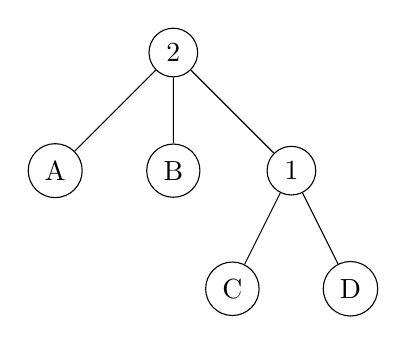
\begin{tikzpicture}
        \scoped{
                \tikzstyle{every node}=[circle, draw];
                \draw (0,0) node (root) [anchor=south] {2} child {node (a) {A}} child {node (b) {B}} child  {node (subroot) {1} child  {node (c) {C}} child  {node (d) {D}}};
            };
    \end{tikzpicture}
    \caption[Sample Access Tree]{
        Sample Access Tree over the attributes \texttt{A}, \texttt{B}, \texttt{C}, \texttt{D}.
    }
    \label{fig:sample-access-tree}
\end{figure}

Explicitly specifying an \gls{access-structure} is not feasible, as its size may be exponential in the size of the attribute universe.
Therefore, we will use the construction of \emph{access trees} defined by Goyal~et~al.~\cite{goyal_attribute-based_2006}.
\Glspl{access-tree} are similar to the tree representation of boolean formulas, but slightly more powerful:
Each leaf of this tree is labelled with an attribute.
Each inner node has a number of children and is labelled with an integer. 
This integer represents the number of children that need to be satisfied in order to satisfy the inner node~\cite{goyal_attribute-based_2006}.

Figure~\ref{fig:sample-access-tree} illustrates an example for an \gls{access-tree}. It is satisfied by any set of attributes that contains two of $A, B$ and either $C$ or $D$.
That is, $\{A,B\}$ would satsify the tree, just as $\{B, D\}$ would, but $\{C, D\}$ would not be sufficient.
For an attribute universe of $U = \{A, B, C, D\}$ this would realize the \gls{access-structure} $\mathcal{A} = \{\{A, B, C, D\}, \{A, B, C\}, \{A, B, D\},\{A, C, D\}, \{B, C, D\}, \{A, B\},\{A, C\},\{A,D\}, \{B, C\},\{B, D\}\}$

\begin{definition}
    Access Tree~\cite{goyal_attribute-based_2006}.

    An interal node $x$ of an \gls{access-tree} is defined by its children and a threshold value $d_x$.
    The threshold value satisfies $0 < d_x \leq num_x$ with $num_x$ being the number of children.
    A leaf node $x$ is defined by an attribute and a threshold value $k_x = 1$.

    The parent of a node $x$ in the \gls{access-tree} is denoted by $\text{parent}(x)$.
    If $x$ is a leaf node, $\text{att}(x)$ denotes the attribute associated with $x$; otherwise it is undefined.
    The children of a node $x$ are numbered from $1$ to $num_x$. Then, $\text{index}(y)$ denotes the unique index of $y$ among the children of its parent node.
\end{definition}

\begin{definition}
    Satisfying Access Trees~\cite{goyal_attribute-based_2006}.

    Let $\mathcal{T}$ be an \gls{access-tree} with root r and $\mathcal{T}_x$ the subtree with $x$ as its root.
    If a set of attributes $\gamma$ satisfies the \gls{access-tree} $\mathcal{T}_x$, we write $\mathcal{T}_x(\gamma) = 1$; otherwise $\mathcal{T}_x(\gamma) = 0$.\\
    If $x$ is a leaf node, then $\mathcal{T}_x(\gamma) = 1$ if and only if $\text{attr}(x) \in \gamma$.
    
    If $x$ is an internal node, then $\mathcal{T}_x = 1$ if and only if $d_x$ or more of the children $x'$ of $x$ return $\mathcal{T}_{x'}(\gamma) = 1$.
\end{definition}
The set of attribute sets that satisfy a tree $\mathcal{T}$ is then the access structure it represents: $\mathcal{A} = \{\gamma \in 2^U | \mathcal{T}(\gamma) = 1\}$.
Note that $\mathcal{A}$ has to be monotone. It is not possible to specify the \emph{absence} of an attribute in the tree.

Using the \gls{access-tree} construction, we can express \emph{A AND B} as a node with two children $A$ and $B$ and threshold $2$, and express \emph{A OR B} as a node with two children $A$ and $B$ and threshold $1$~\cite{yao_lightweight_2015}.

\subsection{Revocation}
So far, it is not possible to take privileges away from a user:
Once the private key has been issued, it can not be taken back.
A user's capabilities can only be extended (e.g. by giving out a key with additional attributes).
This is is a problem, e.g. if their private key is compromised~\cite{boldyreva_identity-based_2008}.

The simplest solution is to simply renew the keys of valid users from time to time~\cite{boldyreva_identity-based_2008}.
When a user is revoked, their key will not be updated any longer. Thus any ciphertexts encrypted after the next key update will not be readable for the revoked user~\cite{boldyreva_identity-based_2008}.
This is inefficient because it requires the \acrshort{kgc} to update or re-issue one key per valid user and needs a secure channel to the \acrshort{kgc}~\cite{boldyreva_identity-based_2008}.

Attrapadung and Imai~\cite{attrapadung_attribute-based_2009} differentiate between \emph{direct} and \emph{indirect revocation}: 
With direct revocation, the list of revoked users is directly specified by the encrypting party (i.e. the encryption takes a ''black list'' of revoked users).
Indirect revocation achieves revocation by means of updating the keys of valid users, as described in the naive approach above.

Direct revocation requires the encryptor to know the list of revoked users \cite{attrapadung_attribute-based_2009} (i.e. the encrypting party is responsible for correct revocation of the users on the revocation list).
This can be a major drawback, especially in large systems or when encryptors are severely constrained (as in our case, \acrshort{iot} devices).
With indirect revocation, the encryptor does not need to do anything except using the most recent version of the public parameters~\cite{attrapadung_attribute-based_2009}.

The advantage of direct revocation, however, is that it works instantly: As soon as an encryptor knows about the revocation of a user, they will include them on their revocation list for future encryptions.
With indirect revocation, a revoked user can decrypt all ciphertexts created until the next key update is distributed by the \acrshort{kgc}~\cite{attrapadung_attribute-based_2009}.

In either case, ciphertexts encrypted before a user's revocation becomes effective, remains readable using the revoked key.
Some schemes include a proxy-reencryption mechanism that allows an untrusted third party to update ciphertexts such that they cannot be decrypted by revoked users~\cite{manna_sea-brew_2021}.


% \subsection{Linear Secret Sharing Schemes and Span Programs}\label{sec:lsss} % reference Shamirs Secret Sharing as an example for LSSS (or the oother way round)
% Instead of the \gls{access-tree} construction, nowadays most \acrshortpl{abes} use monotone \acrfullpl{msp} to describe any \gls{access-structure} realizable by \acrfull{lsss}.
% For a definition of \acrshort{lsss} see~\cite{beimel_secure_1996}.
% Also see there for a proof of the equivalence of \acrshort{lsss} and \acrshort{msp}.

% It is conjectured, but not proven, that there are \glspl{access-structure} that require secret shares of exponential size in any secret sharing scheme that realizes them~\cite{beimel_secure_1996}.
% This would especially mean that not all \glspl{access-structure} can be realized by \acrshort{lsss} (as their shares are smaller than exponential).
% \acrshort{lsss}-realizable \glspl{access-structure} seem to be the most general type of \glspl{access-structure} supported by \acrshortpl{abes} in literature. 

% Any \gls{access-structure} that can be described by an \gls{access-tree} can also be described by a \acrshort{msp} or \acrshort{lsss}.
% For an efficient conversion from Boolean Formulas (which are essentially \glspl{access-tree} limited to two children per inner node) to \acrlongpl{msp}, see the appendix of~\cite{lewko_decentralizing_2011}.
% A more general construction for the threshold trees described in section~\ref{sec:access-trees} is given in~\cite{liu_efcient_2010}.

% \acrshortpl{msp} can realize more general access structures than \glspl{access-tree} and better suited for the design of \acrshortpl{abes}~\cite{agrawal_fame_2017}.

% \begin{definition}
%     (Monotone) Span Program. Adapted from~\cite{goyal_attribute-based_2006, beimel_secure_1996}.\\
%     Let $\mathbb{K}$ be a field and $\{x_1, \dots, x_n,\}$ a set of variables.\\
%     A span program over $\mathbb{K}$ is a labelled matrix $\hat{M} = (M, \rho)$ where $M$ is a matrix over $\mathbb{K}$.
%     $\rho$ is a function that labels every row of $M$ by one literal from $\{x_1, \dots, x_n, \bar{x}_1, \dots, \bar{x}_n\}$.

%     Span programs reject or accept inputs as follows:
%     For an input set $\gamma \subseteq \{x_1, \dots, x_n\}$ let $M_\gamma$ define the submatrix of $M$ consisting only of those rows whose labels are contained in $\gamma$, and the rows labelled by a negated literal $\bar{x}_i$ that is not contained in $\gamma$.
%     That means $M_\gamma$ contains a row $i$ if $\rho(i) = x_j$ and $x_j \in \gamma$ or $\rho(i) = \bar{x}_j$ and $x_j \notin \gamma$.
%     The \acrshort{msp} accepts $\gamma$ if and only if $\vec{1} \in \text{span}(M_\gamma)$, i.e. there exists a linear combination of the rows of $M_\gamma$ that is the row vector consisting of only ones ($\vec{1} = (1, \dots, 1)$).

%     A span program is called \emph{monotone} if the rows are labelled using only the (positive) literals $\{x_1, \dots, x_n\}$.
% \end{definition}

% Note that the vector $\vec{1}$ can be replaced by any other fixed nonzero vector~\cite{beimel_secure_1996}.

% Intuitively, a row $i$ labelled by the literal $\rho(i) = x$ is labelled with the \emph{positive} of $x$; a row labelled by $\rho(i) = \bar{x}$ is labelled by the \emph{negative} of $x$.

% The linear combination yielding $\vec{1}$ may only consist of the rows labelled with positive attributes that are included in $\gamma$ and those labelled with negative literals not included in $\gamma$.
% That means there are coefficients $\{\alpha_i\}_{\rho(i) \in \gamma \text{ or } \rho(i) = \bar{x} \land x \notin \gamma}$ such that $\sum \alpha_i \cdot M_i = \vec{1}$.
% $M_i$ denotes the $i$-th row of the matrix $M$.

% The role of the variables in the definition will be taken by attributes in our context, i.e. each row will be labelled by an attribute or the negation of an attribute~\cite{goyal_attribute-based_2006}.

\section{Shamir's Secret Sharing}
To implement \acrshort{abe}, we need a way to embed secrets in \glspl{access-tree}.
For this, a secret sharing scheme introduced by \citeauthor{shamir_how_1979}~\cite{shamir_how_1979} is used.

Secret sharing schemes allows a secret $s$, which is generally just a number, to be shared among $n$ participants.
The shares are computed such that $s$ can be reconstructed if and only if at least $k$ participants meet and combine their shares.
Such a scheme is then called a $(k,n)$-threshold scheme~\cite{shamir_how_1979}.

\subsection{Lagrange interpolation}
Shamir's scheme makes use of a property of polynomials: A polynomial of degree $d$ is unambiguously determined by $d+1$ points $(x_i, y_i)$.
In other words, any polynomial of degree $d$ can be unambiguously interpolated (reconstructed) from $d+1$ distinct points.

To interpolate a polynomial of degree $d$ from $d+1$ given points $(x_1, y_1), \dots, (x_{d+1}, y_{d+1})$, we can make use of the lagrange basis polynomials:~\cite{yao_lightweight_2015}

\begin{definition}
    Lagrange interpolation: Given a set of $d+1$ points $(x_1, y_1), \dots, (x_{d+1}, y_{d+1})$.

    Then the polynomial 
    \begin{equation}
        L(x) = \sum_{k=0}^d \Delta_{\omega, x_k}(x) \cdot y_k
    \end{equation}
    is the lagrange interpolation polynomial for that set of points, where $\omega = \{x_1, \dots, x_{d+1}\}$ and $\Delta_{\omega,k}(x)$ are the Lagrange basis polynomials:
    \begin{equation}
        \Delta_{\omega,k}(x) = \prod_{\substack{i\in\omega\\ x_i \neq k}} \frac{x-x_i}{x_k-x_i}
    \end{equation}
\end{definition}

This polynomial has degree $d$. If the points $(x_i, y_i)$ lie on a $d$-degree polynomial, then the lagrange interpolation $L(x)$ is \emph{exactly} that polynomial.

On the other hand, if there are less than $d+1$ points of a $d$-degree polynomial known, there are infinitely many $d$-degree polynomials that pass through all given points.~\cite{shamir_how_1979}

% The polynomial can be interpolated unambiguously if at least $k$ points are known, because it has degree $k-1$.
% If only $k-1$ points (or less) are known, there are infinitely many ways to construct a polynomial that passed through all $k-1$ points.
% Therefore, then there are also infinitely many possibilities for $s$.

\subsection{Secret sharing with polynomials}
To share our secret, we now hide it in a polynomial and give out points on this polynomial as secret shares.
Using the lagrange basis polynomials, we can then reconstruct $p(x)$ and thus the secret if we know enough shares~\cite{shamir_how_1979}.

\begin{figure}
    \centering
    \begin{tikzpicture}
        \begin{axis} [axis lines=center, xlabel=$x$, ylabel=$p(x)$, ymin=0]
            \addplot [domain=-0.1:5.05, smooth, thick, color=red] { \PolynomialSSS(x)};
            \fill (axis cs:0,\PolynomialSSS(0)) circle [radius=2pt] node [right] {(0,~s)};
            \fill[color=ForestGreen] (axis cs:1,\PolynomialSSS(1)) circle [radius=2pt] node [right] {(1,~10)};
            \fill[color=ForestGreen] (axis cs:2,\PolynomialSSS(2)) circle [radius=2pt] node [right] {(2,~6)};
            \fill[color=ForestGreen] (axis cs:3,\PolynomialSSS(3)) circle [radius=2pt] node [above] {(3,~2)};
            \fill[color=ForestGreen] (axis cs:4,\PolynomialSSS(4)) circle [radius=2pt] node [right] {(4,~4)};
            \fill[color=ForestGreen] (axis cs:5,\PolynomialSSS(5)) circle [radius=2pt] node [left] {(5,~18)};
          \end{axis}
    \end{tikzpicture}
    \caption[Plot of $(5,4)$-threshold secret sharing scheme]{
        Example for a $(5, 4)$-threshold scheme with $s=8$ and $p(x) = 8 + 7x - 6x^2 + x^3$.
        The five green-colored points are distributed as the secret shares.
        As $p(x)$ has degree three, at least four shares are required to reconstruct $s$.
    }
    \label{fig:sss}
\end{figure}

\begin{definition}
    Shamir's $(k, n)$-threshold secret sharing scheme~\cite{shamir_how_1979}.
    To share a secret $s$ among $n$ participants such that $s$ can be recovered if and only if $k$ or more shares are combined, do:
    \begin{enumerate}
        \item Pick coefficients $a_1, ..., a_{k-1}$ at random 
        \item Set $a_0 = s$. This results in the polynomial $p(x) = a_0 + a_1x + \cdots + a_{k-1}x^{k-1}$. Note that $p(0) = s$.
        \item The secret shares are $(1, p(1)), (2, p(2)), \dots, (n, p(n))$. Give one to each participant.
    \end{enumerate}
    To reconstruct the secret from any subset of $k$ shares, interpolate the polynomial $p(x)$ and evaluate $p(0) = s$. 
\end{definition}

See also Figure~\ref{fig:sss} for illustration.
In practice, the numbers would be far bigger and calculations would not be performed over the real numbers, but rather a finite field modulo a prime~\cite{shamir_how_1979}.

\subsection{Secret Sharing in Attribute Based Encryption}\label{sec:lss-in-access-trees}
To realize an \gls{access-tree} that ``gives away'' a secret if and only if it is satsified by a set of attributes, we can recursively apply Shamir's Secret Sharing scheme:

\begin{figure}
    \centering
    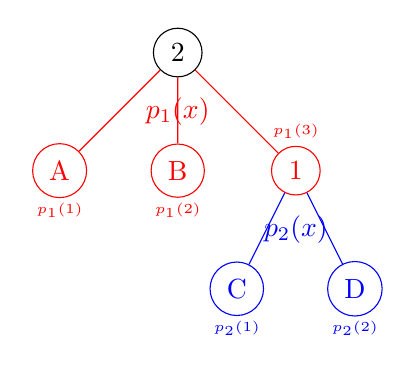
\begin{tikzpicture}
        \scoped{
                \tikzstyle{every node}=[circle, draw];
                \draw (0,0) node (root) [anchor=south] {2} child [red] {node (a) {A}} child [red] {node (b) {B}} child [red] {node (subroot) {1} child [blue] {node (c) {C}} child [blue] {node (d) {D}}};
            };
            \path[red] (root) -- +(0, -0.75) node {$p_1(x)$};
            \path[red] (a) -- +(0, -0.5) node {\tiny$p_1(1)$};
            \path[red] (b) -- +(0, -0.5) node {\tiny$p_1(2)$};
            \path[red] (subroot) -- +(0, 0.5) node {\tiny$p_1(3)$};

            \path[blue] (subroot) -- +(0, -0.75) node {$p_2(x)$};
            \path[blue] (c) -- +(0, -0.5) node {\tiny$p_2(1)$};
            \path[blue] (d) -- +(0, -0.5) node {\tiny$p_2(2)$};
    \end{tikzpicture}
    \caption[Shamir's Secret Sharing in Access Trees]{
        \Gls{access-tree} from Figure~\ref{fig:sample-access-tree} showing how Shamir's secret sharing is employed recursively.
        $p_1(x)$ is a the polynomial of a $(2,3)$-threshold scheme, $p_2(x)$ of a $(1,2)$-threshold scheme.
        Shown in small are the secret shares embedded into each node.
    }
    \label{fig:sample-access-tree-shamir}
\end{figure}

We use a secret-sharing polynomial on each internal node of the \gls{access-tree}.
For a node $x$ with threshold $d_x$ and $\text{num}_x$ children, we define a $(d_x, \text{num}_x)$-threshold scheme and embed one share of the secret in each child.
We begin in the root, and set $s$ as the secret we want to embed in the tree.
For all other nodes, we set $s$ as the secret share received from the parent node.

If the child is a leaf, we modify the share such that it can only be used if the relevant attribute is present (how exactly this is done differs between \acrshort{cp-abe} and \acrshort{kp-abe}).

Now, let $\omega$ be a set of attributes.
We have built our tree in such a way that the share embedded in a leaf node $u$ can be used only if $\text{attr}(u) \in \omega$.
That means, a leaf node's secret share can be used if and only if the set of attributes satisfies this leaf node.

For the internal nodes $x$, the use of a $(d_x, \text{num}_x)$-threshold scheme ensures that the secret embedded in $x$ can be reconstructed if and only if the secret shares of at least $d_x$ child nodes can be used, i.e. at least $d_x$ child nodes are satisfied.
Following this recursive definition up to the root, we can see that our secret $s$ embedded in the root can be reconstructed if and only if $\omega$ satisfies the acess tree.

See Figure~\ref{fig:sample-access-tree-shamir} for an illustration with the tree from Figure~\ref{fig:sample-access-tree}:
Two $(k,n)$-threshold schemes are employed, one for each internal node of the \gls{access-tree}.
$p_1(x)$ is the polynomial of the root's $(2,3)$-threshold scheme, sharing $s$, the secret to be embedded in the tree (i.e. $p_1(0) = s$).
$p_2(x)$ is the polynomial for the $(1,2)$-threshold scheme belonging to the node labelled ``1'' and shares the value $p_1(3)$ that it received from the $(2,3)$-threshold scheme of the layer above (i.e. $p_2(0) = p_1(3)$).

\section{Elliptic Curves}
\label{sec:ec}

The mathematics of modern cryptosystems (including, but not limited to ABE) work any group that satisfies the axioms (see below), and \glspl{ec} are just one of them.
Because \Glspl{ec} allow for shorter key lengths than, e.g. groups modulo a prime, they have become very popular for use in cryptography.
Exact definitions and notations differ, these are taken from the textbook \emph{Introduction to Modern Cryptography} by Katz and Lindell~\cite{katz_introduction_2015}.

\subsection{Group Axioms}\label{sec:group}
\begin{definition}~\cite{katz_introduction_2015}. A \emph{Group} $\langle \mathbb{G}, \circ, e \rangle$ consists of a set $\mathbb{G}$ together with a binary operation $\circ$ for which these four conditions hold:
    \begin{itemize}
        \item Closure: For all $g, h \in \mathbb{G}$, $g \circ h \in \mathbb{G}$.
        \item Existence of identity: There is an element $e \in \mathbb{G}$, called the \emph{identity}, such that for all $g \in \mathbb{G}$, $g \circ e = g = e \circ g$.
        \item Existence of inverse: For every $g \in \mathbb{G}$ there exists an \emph{inverse} element $h \in \mathbb{G}$ such that $g \circ h = e = h \circ g$.
        \item Associativity: For all $g_1, g_2, g_3 \in \mathbb{G}$, $(g_1 \circ g_2) \circ g_3 = g_1 (\circ g_2 \circ g_3)$.
    \end{itemize}
    If $\mathbb{G}$ has a finite number of elements, the group $\mathbb{G}$ is called finite and $|\mathbb{G}|$ denotes the order of the group.

    A group $\mathbb{G}$ with operation $\circ$ is called \emph{abelian} or commutative if, in addition, the following holds:
    \begin{itemize}
        \item Commutativity: For all $g, h \in \mathbb{G}, g \circ h = h \circ g$.
    \end{itemize}

    When the binary operation is clear from context, we simply use $\mathbb{G}$ to denote the group.

    We also define \emph{Group Exponentiation}: $g \in \mathbb{G}, m \in \mathbb{N}^+$, then $mg = \underbrace{g \circ \cdots \circ g}_{m \text{ times}}$.
\end{definition}


Usually, the symbol used to denote the group operation is not the $\circ$ from above, but either $+$ or $\cdot$. These are called \emph{additive} and \emph{multiplicative} notation, respectively.
It is important to remember, though, that the group operation might be defined completely differently!

In multiplicative notation, the group exponentiation of $g \in \mathbb{G}$ with $m \in \mathbb{N}^+$ is written as $g^m$, in additive groups it is written as $m \cdot g$.

An example for an additive group is $\langle \mathbb{Z}_N, +_N, 0 \rangle$ with $\mathbb{Z}_N = \{0, 1, \dots, N-1\}$ and $+_N$ the normal addition modulo $N$.
This group is cyclic with generator $1$.
If $p$ is prime, then $\langle \mathbb{Z}^*_p, \cdot_p, 1 \rangle$ is a group with $\mathbb{Z}^*_p = \{k \in \mathbb{Z}_p | \text{gcd}(k,p) = 1\}$ and $\cdot_p$ the normal multiplication modulo $p$.

\subsection{Elliptic Curves}

\begin{definition}
    Given a prime $p \geq 5$ and $a, b \in \mathbb{Z}_p$ with $4a^2 + 27b^2 \neq 0 \bmod{p}$, the \gls{ec} over $\mathbb{Z}_p$ is~\cite{katz_introduction_2015}:
    \begin{equation}
        E(\mathbb{Z}_p) := \{(x, y)~|~x,y \in \mathbb{Z}_p \text{ and } y^2 = x^3 + a x + b \bmod{p}\} \cup \{\mathcal{O}\}
    \end{equation}
\end{definition}

$a$ and $b$ are called the curve parameters, and the requirement that $4a^2 + 27b^2 \neq 0 \bmod{p}$ makes sure that the curve has no repeated roots~\cite{katz_introduction_2015}.
The curve is simply the set of points $(x, y) \in \mathbb{Z}_p \times \mathbb{Z}_p$ that satisfy the curve equation $y^2 = x^3 + a x + b \bmod{b}$.
One special point is added, the \emph{point at infinity} denoted by $\mathcal{O}$.
This will help define the point addition as a group operation in the next paragraph~\cite{katz_introduction_2015}.

\subsection{Point Addition}
Now, it is possible to show that every line intersecting a curve $E(\mathbb{Z}_p)$ intersects it in exactly three points, if you (1) count tangential intersections double and (2) count any vertical line as intersecting the curve in the point at infinity $\mathcal{O}$~\cite{katz_introduction_2015}.
Therefore, $\mathcal{O}$ can be thought of as sitting ``above'' the end of the y-axis~\cite{katz_introduction_2015}.
Figure~\ref{fig:ecc-point-addition} shows the four different cases.

Using this intersecting line, we can define an operation on curve points:
\begin{definition}
    \label{def:point-add}
    Given an \gls{ec} $E(\mathbb{Z}_p)$, we define a binary operation called \emph{(point) addition} and denoted by $+$:~\cite{katz_introduction_2015}\\
    Let $P_1, P_2 \in E(\mathbb{Z}_p)$.

    \begin{itemize}
        \item For two points $P_1, P_2 \neq \mathcal{O}$ and $P_1 \neq P_2$, their sum $P_1 + P_2$ is evaluated by drawing the line through $P_1$ and $P_2$. 
            This line will intersect the curve in a third point, $P_3 = (x_3, y_3)$.
            Then the result of the addition is $P_1 + P_2 = (x_3, -y_3)$, i.e. $P_3$ is reflected in the $x$-axis (Figure~\ref{fig:ecc-point-addition}-1).
            If $P_3 = \mathcal{O}$, then the result of the addition is $\mathcal{O}$ (Figure~\ref{fig:ecc-point-addition}-3).
        \item If $P_1, P_2 \neq \mathcal{O}$ and $P_1 = P_2$, as above but draw the line as tangent on the curve in $P_1$ (Figure~\ref{fig:ecc-point-addition}-2 and -4).
        \item If $P_1 = \mathcal{O}$, then $P_1 + P_2 = P_2$ and vice-versa.
    \end{itemize}
\end{definition} 

\begin{figure}
    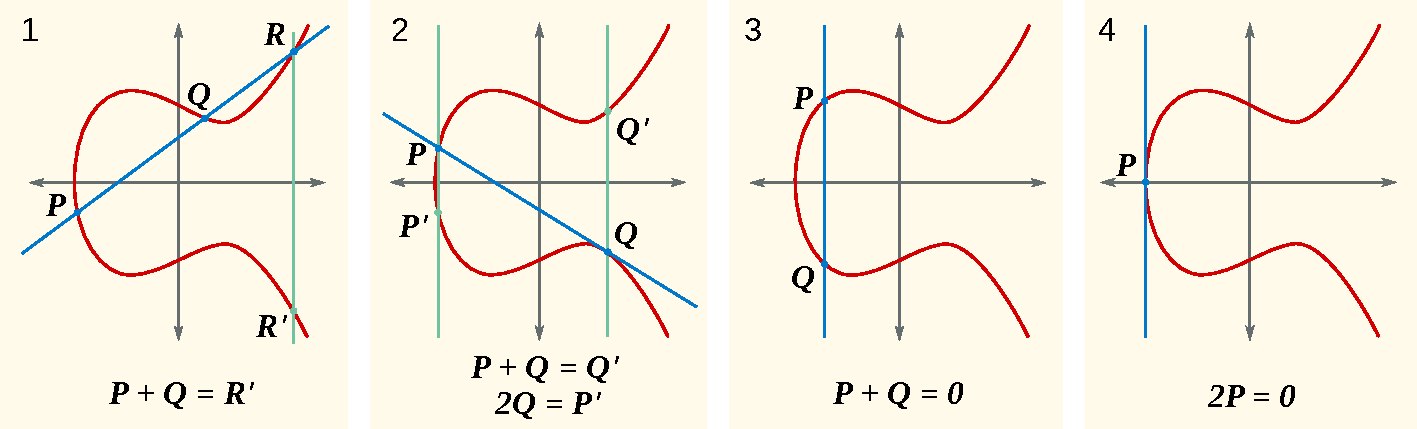
\includegraphics[width=\textwidth]{figures/ecc_point_addition.pdf}
    \caption[Elliptic curve point addition]{Elliptic curve point addition\\(Image by \href{https://commons.wikimedia.org/wiki/File:ECClines-2.svg}{SuperManu}, licensed under \href{https://creativecommons.org/licenses/by-sa/3.0/deed.en}{Creative Commons}.)}
    \label{fig:ecc-point-addition}
\end{figure}

We will be adding points to themselves a lot. Therefore, we define for ease of notation:
\begin{definition}
    Point-Scalar multiplication: Given a point $P \in E(\mathbb{Z}_p)$ and a scalar $d \in \mathbb{N}$: 
    \begin{equation}
        d \cdot P = \underbrace{P + P + \cdots + P}_{d \text{ times}}
    \end{equation}
\end{definition}
 
That is exactly the definition of group exponentiation, applied to our additive \gls{ec} group. Note that the product of a scalar with a point is again a point on our curve.\\

\subsection{Groups on Elliptic Curves}
\begin{theorem}
    The points of an \gls{ec} $E(\mathbb{Z}_p)$ plus the addition law as stated in Definition~\ref{def:point-add} form an abelian (commutative) group~\cite{katz_introduction_2015, washington_elliptic_2008}:
\end{theorem}
\begin{proof}
    A formal proof is outside the scope of this thesis, but here's some informal reasoning about the group axioms:
    \begin{itemize}
        \item Existence of Identity: $P + \mathcal{O} = P$ (as per definition)
        \item Commutativity: For all $P_1, P_2 \in E(\mathbb{Z}_p)$, $P_1 + P_2 = P_2 + P_1$ (because the line through $P_1$ and $P_2$ will be the same)
        \item Unique inverse: For all $P = (x,y) \in E(\mathbb{Z}_p)$, the unique inverse is $-P = (x, -y)$ (because the line through $P$ and $-P$ will be vertical).
        \item Associativity: For all $P_1, P_2, P_3 \in E(\mathbb{Z}_p)$, $(P_1 + P_2) + P_3 = P_1 + (P_2 + P_3)$ (much less obvious, see e.g.~\cite[chapter 2.4]{washington_elliptic_2008} for a proof).
    \end{itemize}
\end{proof}

Of particular interest to cryptography are \emph{cyclic} groups on \glspl{ec}:
\begin{definition}
    An (additive) group $\mathbb{G}$ is cyclic if there is an element $g \in \mathbb{G}$ that generates $\mathbb{G}$, i.e. $\mathbb{G} = \langle g \rangle = \{k \cdot g | k \in \mathbb{Z}\}$.
\end{definition}

Translated to our \glspl{ec}, this means that there is a generator point $P \in E(\mathbb{Z}_p)$, such that every point $Q \in E(\mathbb{Z}_p)$ can be obtained by repeatedly adding $P$ to itself using the point addition from Definition~\ref{def:point-add}.

\begin{theorem}\cite{katz_introduction_2015}
    Let $\mathbb{G}$ be a finite group of order $n$, i.e. $|\mathbb{G}| = n$.
    Let $g \in \mathbb{G}$ be an element of $\mathbb{G}$ with order $k$, i.e. $k = |\langle g \rangle |$

    Then $k|n$, i.e. the order of $g$ divides the group order $n$.
\end{theorem}
\begin{proof}
    See \cite*[Proposition 8.54]{katz_introduction_2015}.
\end{proof}

There is an important consequence to this fact: If a group has prime order, all points except the identity are generators.
This stems from the fact that a prime number has exactly two divisors: One (the order of the identity) and itself (the order of all other points).

Again, translated to \glspl{ec} this means that if the number of points $\#E(\mathbb{Z}_p)$ on a curve is prime, all points except $\mathcal{O}$ are generators.
These cyclic \gls{ec} groups are exactly the groups we are interested in for doing actual cryptography.
The ease of finding generators is one reason, but not the only one. 
For a detailed explanation, see \cite[p.~321]{katz_introduction_2015}.

% \subsection{Hardness Assumptions}

% Most ECC schemes are build upon three hardness assumptions: The Discrete Logarithm Problem (DLP), the Decisional Diffie-Hellman Problem (DDHP) and the Computational Diffie-Hellman Problem (CDHP).
% Given an additive, cyclic group $\mathbb{G}$ with $P \in \mathbb{G}$ a generator, they are stated as follows:
% \\

% \emph{Discrete Logarithm Problem.} Given an arbitrary point $Q \in \mathbb{G}$, compute an $n \in \mathbb{N}$ such that $n P = Q$. % n from Zq?

% \emph{Computational Diffie-Hellman Problem.} Given the triple $(P, aP, bP)$ where $a, b \in \mathbb{N}$ chosen uniformly at random, compute $abP$.

% \emph{Decisional Diffie-Hellman Problem.} Given two triples $(aP, bP, abP)$ and $(aP, bP, Q)$ where $a, b \in \mathbb{N}$ and $Q \in \mathbb{G}$ chosen uniformly at random, distinguish between the two.
% \\

% Now, the hardness \emph{assumption} is that, for some groups, these problems are hard to solve, i.e. solving them requires so much time and computational power that it is infeasible.
% From this, we can build secure asymmetric encryption schemes.

% These three problems might all be assumed to be \emph{hard}, but that doesn't mean they are equally so:
% If, in a certain group $\mathbb{G}$, the DLP problem is easy, so is CDHP: Just compute $a$ and $b$, and then use them to calculate $abP$.
% And if CDHP is easy w.r.t some $\mathbb{G}$, so is DDHP: Just compute $abP$, and compare the third element of each tuple.
% The inverse is not generally true, i.e. there are groups in which DLP and CDHP are hard to solve, even though DDHP is easy to solve.
% In that sense, DLP is the hardest and DDHP the easiest of the three. \cite{katz_introduction_2015} (find out if this is true. \cite{menezes_introduction_2009})

\subsection{Bilinear Pairings}\label{sec:bilinear-pairings}

\begin{definition}Bilinear pairing~\cite{kiraz_still_2016}.\\
    Let $\mathbb{G}_1$ and $\mathbb{G}_2$ denote cyclic groups with prime order $n$.
Let $\mathbb{G}_T$ be another cyclic group of the same order $n$. 
$\mathbb{G}_1$ and $\mathbb{G}_2$ are written additively, $\mathbb{G}_T$ is written using multiplicative notation.\\
    A \emph{bilinear pairing} then is a function $e: \mathbb{G}_1 \times \mathbb{G}_2 \rightarrow \mathbb{G}_T$ with the following properties:
    \begin{itemize}
        \item \emph{Bilinearity.} For all $P_1, P_2 \in \mathbb{G}_1, Q_1, Q_2 \in \mathbb{G}_2$
        \begin{itemize}
            \item $e(P_1+P_2, Q_1) = e(P_1,Q_1)\cdot e(P_2,Q_1)$
            \item $e(P_1, Q_1+Q_2)=e(P_1,Q_1)\cdot e(P_1,Q_2)$
        \end{itemize}
        \item \emph{Non-Degeneracy.}
        \begin{itemize}
            \item for each $P \in \mathbb{G}_1, P \neq 0$ there is a $Q \in \mathbb{G}_2$ with $e(P, Q) \neq 1$
            \item for each $Q \in \mathbb{G}_2, Q \neq 0$ there is a $P \in \mathbb{G}_1$ with $e(P, Q) \neq 1$
        \end{itemize}
        \item \emph{Computability.} There is an algorithm that computes $e$ efficiently.
    \end{itemize}
    If $\mathbb{G}_1 = \mathbb{G}_2$, the pairing is called a \emph{symmetric pairing}, otherwise it is an \emph{asymmetric pairing}.
\end{definition}

There are a few different concrete pairing functions, e.g. the Weil pairing, Tate pairing and the Ate pairing~\cite{kiraz_still_2016}.
Usually the source groups $\mathbb{G}_1$ and $\mathbb{G}_2$ are subgroups of certain \glspl{ec} \cite{kiraz_still_2016} and the target $\mathbb{G}_T$ is a finite field (\emph{not} another point on a curve)~\cite{blake_advances_2005}.

\subsection{Use of elliptic curves and pairings in ABE}
Elliptic curves are already widely used in \glslink{pkes}{asymmetric cryptography}.
Bilinear pairings, on the other hand, are relatively new and have given rise to a whole new class of cryptographic algorithms, the \emph{pairing-based cryptography}.
For example, pairings are used to construct \gls{ibe}, a three-party \gls{dh}~\cite{joux_one_2000} or short \glspl{dss}~\cite{boneh_short_2001}.

Most \acrshortpl{abes} make use of bilinear pairings, and even pairing-free schemes (see next section) need an implementation of the \gls{ec} operations.
These operations are the building blocks of the \acrshortpl{abes} presented in chapter~\ref{chapter:constructions} and by far the most expensive operations performed by the schemes.
Therefore, the performance of an \acrshort{abe} implementation greatly depends on the performance of the \gls{ec} and pairing implementation.
For this reason, pairing implementations are considered in chapter~\ref{chap:related-work} and our own pairing implementation is evaluated separately in chapter~\ref{chap:evaluation}.